\subsubsection{Eliminierung 3 bis 5 Harmonischer}
\label{6_2_title}

Bei diesem Verfahren wurde die dritte und fünfte Harmonische eliminiert. Da es sich hierbei um einen zweiphasigen Wechselrichter handelt, ist die dritte Harmonische nicht automatisch eliminiert.\\

Um zwei Harmonische eliminieren zu können, muss das Steuersignal zwei Freiheitsgrade aufweisen.


\begin{figure}[H]
  \begin{center}
  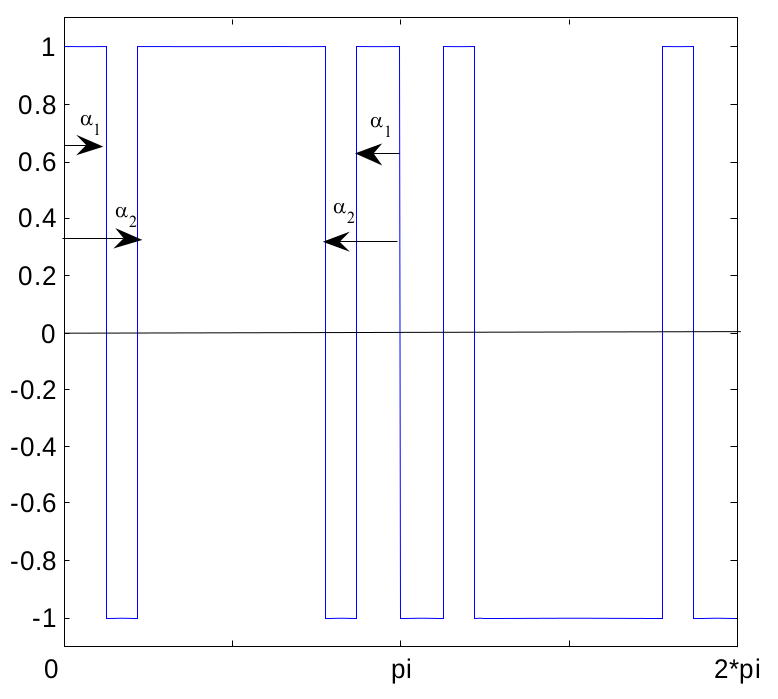
\includegraphics[width=0.48\textwidth]
  {pic/6_2_weitere_pulsmuster/6_2_1_stromform/freiheitsgrade.png}
  \caption{$Zwei Freiheitsgrade$}
  \label{fig:6_2_freiheitsgrade}
  \end{center}
\end{figure}

Durch Berechnen von $\alpha_1$ und $\alpha_2(\alpha_1)$ können bestimmte harmonische entfernt werden, in unserem Fall die dritte und fünfte.


\clearpage
%
% KO Pictures
%
Das Ansteuerungssignal in Abbildung \ref{fig:6_2_1_0} sieht gleich aus wie in Abbilung \ref{fig:6_2_freiheitsgrade}.
\begin{figure}[H]
  \begin{center}
  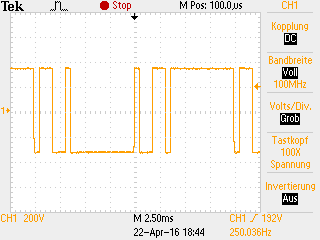
\includegraphics[width=0.48\textwidth]
  {pic/6_2_weitere_pulsmuster/6_2_1_stromform/eliminierung_3_bis_5/ALL0000/F0000TEK.png}
  \caption{$U_A (Orange)$}
  \label{fig:6_2_1_0}
  \end{center}
\end{figure}

Die violette Kurve entspricht: $U_L = U_A - U_{Netz}$
\begin{figure}[H]
  \begin{center}
  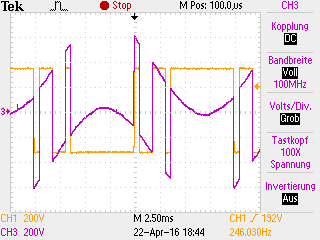
\includegraphics[width=0.48\textwidth]
  {pic/6_2_weitere_pulsmuster/6_2_1_stromform/eliminierung_3_bis_5/ALL0001/F0001TEK.png}
  \caption{$U_A (Orange), U_L (Violett)$}
  \label{fig:6_2_1_1}
  \end{center}
\end{figure}
\clearpage 

Der Stromverlauf $I_{L1}$ richted sich nach der Spannung $U_L$. Der Kurvenverlauf von $I_{L1}$ ist sehr gut ersichtlich anhand des Integrales, $I_L = \frac{1}{L} \int U_L dt$.
\begin{figure}[H]
  \begin{center}
  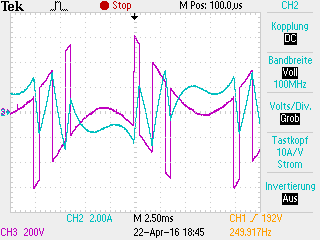
\includegraphics[width=0.48\textwidth]
  {pic/6_2_weitere_pulsmuster/6_2_1_stromform/eliminierung_3_bis_5/ALL0002/F0002TEK.png}
  \caption{$U_L (Violett), I_{L1} (Hellblau)$}
  \label{fig:6_2_1_2}
  \end{center}
\end{figure}

Bei der Messung war ersichtlich, dass der Anteil der dritten und fünften Harmonischen kleiner als 1\% war. Dieses Prozent kann durch Messfehler verursacht werden, sowie durch nicht exaktes einhalten von $\alpha_1$ und $\alpha_2$

\clearpage